\documentclass[12pt,a4paper]{article}
\usepackage{graphicx}
\usepackage[english]{babel}
\usepackage[T1]{fontenc}
\usepackage[utf8]{inputenc}
\usepackage{verbatim}
\usepackage[hidelinks]{hyperref}
\usepackage{bookmark}
\usepackage{listings}
\usepackage{amsmath}
\usepackage{amssymb}
\usepackage{amsthm}
\usepackage{ae,aecompl}

\newcommand{\leftexp}[2]{{\vphantom{#2}}^{#1}{#2}}
\newcommand{\leftsub}[2]{{\vphantom{#2}}_{#1}{#2}}

\theoremstyle{plain}% default
\newtheorem{thm}{Theorem}[section]
\newtheorem{lem}[thm]{Lemma}
\newtheorem{prop}[thm]{Proposition}
\newtheorem*{cor}{Corollary}

\theoremstyle{definition}
\newtheorem{defn}{Definition}[section]
\newtheorem{conj}{Conjecture}[section]
\newtheorem{exmp}{Example}[section]

\theoremstyle{remark}
\newtheorem*{rem}{Remark}
\newtheorem*{note}{Note}
\newtheorem{case}{Case}



\begin{document}

\title{Application of D-symbols on edge transitive tilings}
\author{Boróczki, Lajos}
\maketitle
%\tableofcontents

\begin{abstract}
  Any tiling, generated by a crystallographic group with compact fundamental
  domain, can be represented by a diagram and a matrix function, based on
  their barycentric subdivision and the adjacency relations between the orbits
  and the particular simplices. The representation is called the D-symbol of a
  tiling in honour of B. N. Delone, M.S. Delaney and A.W.M. Dress. The
  representation is easily adoptable to computer programs.

  After a short introduction and definition of D-symbols we 
  present some recent results of edge transitive D-symbols and some of their
  nice properties found by computer analysis.
\end{abstract}

\section{Introduction}
This work is based on...

Why D-symbol?

Unpublished accomplishments?

Why just some examples?

\section{D-symbols}
We shall briefly introduce D-symbols (for a more comprehensive introduction see
also \cite{BSzK02}, \cite{DHM93}, \cite{M96}, stb.\footnote{FIXME}). 

For an equivariant periodic tiling $(\mathcal{T},\Gamma)$ in a $d$-dimensional
simply connected manifold $\mathcal{S}^d$ (with its piece-wise linear (PL)
topology) the barycentric simplex subdivision of $\mathcal{T}$ can be taken,
which remains compatible with the group action of $\Gamma$. Let's denote the
resulting chamber system by $\mathcal{C}$, the $\Gamma$ orbit of a chamber $C\in
\mathcal{C}$ by $D=C^\Gamma$, and $\mathcal{D}:= \mathcal{C}^\Gamma$ the set of
chamber orbits. Every $C\in \mathcal{C}$ is a $d$-dimensional simplex, and the
vertices of the simplex can be labeled by the numbers $0,\ldots,d$ showing the
dimension of their respective face centered in the corresponding vertex. For
example if we take the baricentric subdivision of a $3$-dimensional cube: we get
a body center labeled by $3$, a facet center labeled by $2$, an edge center
labeled by $1$ and one of the original vertices labeled by $0$. The facets of
the chambers ($d-1$-dimensional faces) can be labeled by the same $0,\ldots,d$
using the label of the only vertex, that the facet doesn't contain.

Every chamber has $d+1$ neighbours by the facet they share and this adjacency is
preserved by the action of $\Gamma$. So we can take the adjacency operations and
use them formally as a free Coxeter group $\Sigma^I := <(\sigma^i, i\in I) |
((\sigma^i)^2=1, i\in I)>$ acting on $\mathcal{C}$ and on $\mathcal{D}$
respectively, where $I$ is the index set of $0,\ldots,d$. 

\begin{note}
  It's possible to get back to a starting chamber (or later its orbit) if we
  take a route $\sigma^i\sigma^j\ldots\sigma^i\sigma^j(C) = C$ around an
  $ij$-edge of the starting chamber C.
\end{note}

\begin{note}
  We write $\sigma^iC^\phi=(\sigma^iC)^\phi=\sigma^i(C^\phi)$ for
  $\sigma^i\in\Sigma^I$ and $\phi\in\Gamma$, indicating that the adjacencies are
  invariant under the symmetry group $\Gamma$.
  
  So if a geometric mapping on a point(set) acts on the right (as in our
  convention), then $\Sigma^I$ acts on the left, as a formal associative
  law.\footnote{FIXME Ez a kifejezes mit is jelent magyarul? Meg nem talalkoztam
  vele.}
\end{note}

\begin{note}
(As we only consider periodic tilings, which means $\mathcal{D}$ is
finite,\footnote{FIXME a periodic tiling definiciojaban nem pont ez van benne?} this
automatically defines some relations of $\Sigma^I$ and so of $\Gamma$ affecting
$\mathcal{D}$ and vice versa.)\footnote{FIXME Ezt az egesz megjegyzest
kihagynam, egy nem tul fontos algebrai megjegyzest probaltam volna atadni,
miszerint ha egy szabad csoportot egy veges halmazon hattatok, akkor emiatt biztosan
vannak relaciok.}
\end{note}

Next we have to deal with these relations. We require that the following
relations hold for every $C\in\mathcal{C}$ (and every $C^\Gamma=D\in\mathcal{D}$
respectively):
\begin{itemize}
  \item For every $i,j\in I$, where $|i-j|=1$, there exists
    $m\in\mathbb{N}^+$:
    $(\sigma^j\sigma^i)^mC=(\sigma^i\sigma^j)^mC=C$, lets denote the smallest
    possible $m$ value by $m^{ij}(C)=m^{ji}(C)$.
  \item For every $i,j\in I$, where $|i-j|>1$:
    $(\sigma^j\sigma^i)^2C=(\sigma^i\sigma^j)^2C=C$, $m^{ij}(C)=m^{ji}(C)=2$,
    in compatibility with the baricentric subdivision.  
  \item (For every $i\in I$: $(\sigma^i)^2C=C$, $m^{ii}(C)=1$, which has already
    been naturally defined.)
\end{itemize}

We can introduce the matrix function $\mathcal{M}: \mathcal{C}
\rightarrow \mathbb{N}^{(d+1)\times (d+1)}$: $\mathcal{M}(C)^{i,j}=m^{ij}(C)$, which
gives us half the number of chambers around an $ij$-edge. Notice that $\mathcal{M}$
will be the same for the orbits ($\mathcal{D}$), as requirement, expressing that
the action of $\Gamma$ doesn't change the number of chambers around a given
edge.

Similarly one can define the $\mathcal{R}$ matrix function for the
relations of the $\Gamma$ orbits of the chambers ($\mathcal{D}$), which gives us
half the number of chamber-orbits around an edge. Every entry of the $\mathcal{R}$
matrix function has to divide the respective entry of $\mathcal{M}$ for
every $D\in\mathcal{D}$. Namely, for every $i,j\in I$ exists the value $r$ such that
$(\sigma^j\sigma^i)^rD=(\sigma^i\sigma^j)^rD=D$. Lets denote the smallest
possible $r$ value by $r^{ij}(D)=r^{ji}(D)$. There exists $C\in\mathcal{C}$ so
that $D=C^\Gamma$.
\begin{align}
  |i-j|=1 & \Rightarrow r^{ij}(D)|m^{ij}(C) \\
  |i-j|>1 & \Rightarrow 1\leq r^{ij}(D)\leq 2 \\
  i=j & \Rightarrow r^{ij}(D)=1
\end{align}

Let $v^{ij}(D)$ the following: $m^{ij}(D)=r^{ij}(D)v^{ij}(D)$ and
let's define the valence matrix function
$\mathcal{V}(D)^{i,j}=v^{ij}(D)$.

%It's easy to see that the values of both matrix functions must be the
%same around an edge ($D,D'\in\mathcal{D}$, $C,C'\in\mathcal{C}$, $i,j\in I$,
%$a\in {0,1}$, $b\in \mathbb{N}$):
%\begin{align}
%  D'=(\sigma^i)^a(\sigma^i\sigma^j)^b(D) & \Rightarrow
%  \mathcal{R}(D)^{i,j}=\mathcal{R}(D')^{i,j} \\
%  D'=(\sigma^i)^a(\sigma^i\sigma^j)^b(D) & \Rightarrow
%  \mathcal{M}(D)^{i,j}=\mathcal{M}(D')^{i,j} \\
%  C'=(\sigma^i)^a(\sigma^i\sigma^j)^b(C) & \Rightarrow
%  \mathcal{M}(C)^{i,j}=\mathcal{M}(C')^{i,j}
%\end{align}

If we take a small ball around every chamber-vertex (so small, that it doesn't
contain another chamber vertex), then the tiling on the boundary of the ball
induced by the original tiling must be an $S^{d-1}$ tiling \cite{D87} if the
chamber vertex is a proper one (not an ideal vertex (in infinity) or an
out-of-model vertex).

The triplet $(\Sigma^I,\mathcal{D},\mathcal{M})$ is called the D-symbol of a
tiling in honour of Delone, Delaney and Dress. A main consequence is the
following theorem \cite{D87}.
\begin{thm}
$(\mathcal{T},\Gamma)$ and
$(\mathcal{T}',\Gamma')$ are equivalent (topologically equivariant (homeomeric))
if and only if the correspondig $(\Sigma^I,\mathcal{D},\mathcal{M})$ and
$(\Sigma^I,\mathcal{D}',\mathcal{M}')$ D-symbols are isomorphic.
\end{thm}

\section{The inverse problem}
Our main concern is the inverse problem: Which triplets
$(\Sigma^I,\mathcal{D},\mathcal{M})$ exist with some nice constraints and how
can we find the orbifold and the geometry which realizes it by an equivariant tiling
$(\mathcal{T},\Gamma)$?

Let's recall the definitions and theorems used in this paper.
\begin{defn}
  A $d$-dimensional {\em D-diagram} is a $d+1$ colored connected graph of the
  adjacency operations $(\Sigma^I,\mathcal{D})$. Where $|I|=d+1$,
  $|\mathcal{D}|$ is the finite {\em cardinality} of the diagram, for every $i\in
  I$ $(\sigma^i)^2=1$ and for every $i,j\in I$ if $|i-j|>1$ then
  $(\sigma^i\sigma^j)^2D=D$. We use the following colors on our figures up to 3
  dimensions:

  \setlength{\unitlength}{1cm}
  $\sigma^0$:
  \begin{picture}(1,0.2)
    \multiput(0,0.1)(0.2,0){5}{\circle*{0.001}}
  \end{picture},
  $\sigma^1$:
  \begin{picture}(1,0.2)
    \multiput(0,0.1)(0.25,0){4}{\line(1,0){0.15}}
  \end{picture},
  $\sigma^2$:
  \begin{picture}(1,0.2)
    \put(0,0.1){\line(1,0){1}}
  \end{picture},
  $\sigma^3$:
  \begin{picture}(1.5,0.2)
    \multiput(0,0.1)(0.5,0){3}{\line(1,0){0.2}}
    \multiput(0.35,0.1)(0.5,0){3}{\circle*{0.001}}
  \end{picture}
\end{defn}

\begin{defn}
  {\em The matrix function $\mathcal{R}$.}
  Let $\mathcal{R}$: $\mathcal{D} \rightarrow \mathbb{N}^{(d+1)\times (d+1)}$.
  For every $D\in\mathcal{D}$, for every $i,j\in I$ there exists $r\in
  \mathbb{N}\setminus \{0\}$ such that
  $(\sigma^j\sigma^i)^rD=(\sigma^i\sigma^j)^rD=D$ ($|\mathcal{D}|<\infinity$).
  $\mathcal{R}(D)^{i,j}:=r$
\end{defn}
  
\begin{defn}
  {\em The matrix function $\mathcal{M}$.}
  Let $\mathcal{M}$: $\mathcal{D} \rightarrow \mathbb{N}^{(d+1)\times (d+1)}$.
  For every $D\in\mathcal{D}$, for every $i,j\in I$:
  \begin{align}
    i=j & \Rightarrow \mathcal{M}(D)^{i,i}=1 \\
    |i-j|>1 & \Rightarrow \mathcal{M}(D)^{i,j}=2 \\
    |i-j|=1 & \Rightarrow \mathcal{R}(D)^{i,j}|\mathcal{M}(D)^{i,j}
  \end{align}
  The only interesting values of the matrix function are at the subdiagonals, so
  we can use the following shorter notation:
  $D_1(\mathcal{M}(D_1)^{0,1},\ldots,\mathcal{M}(D_1)^{d,d+1})$, $\ldots$,
  $D_{|\mathcal{D}|}(\mathcal{M}(D_{|\mathcal{D}|})^{0,1},\ldots,\mathcal{M}(D_{|\mathcal{D}|})^{d,d+1})$
\end{defn}

\begin{defn}
  {\em The matrix function $\mathcal{V}$ of valences as rotational orders
  as parameters.}
  Let $\mathcal{V}$: $\mathcal{D} \rightarrow \mathbb{N}^{(d+1)\times (d+1)}$.
  $\mathcal{M}(D)=\mathcal{R}(D)\mathcal{V}(D)$.
\end{defn}

\begin{defn}
  We call the triplet $(\Sigma^I,\mathcal{D},\mathcal{M})$ {\em D-symbol}, if the
  following additional constraint is met:
  $\forall D\in \mathcal{D}$, $\forall i,j\in I$, $\forall a\in {0,1}$,
      $\forall b\in \mathbb{N}$: if $D'=(\sigma^i)^a(\sigma^i\sigma^j)^b(D)$,
      then $\mathcal{M}(D)^{i,j}=\mathcal{M}(D')^{i,j}$, namely the
      $\mathcal{M}$ matrix function has the same values around edges.\footnote{FIXME:
      Mivel ezt az elejen csak bevezetes szinten emlegettem, szerintem szukseges
      a defincios reszben kulon kiterni ra, persze lehet, hogy nem ebben a
      cikkben.}
\end{defn}

%\begin{defn}
%  Based on the previous definition one can define the {\em parametric D-symbol} of
%  a given D-diagram, which has a parametric $\mathcal{M}$ matrix function,
%  which is the same for every $D\in\mathcal{D}$, for every $i,j\in I$ when
%  $|i-j|\neq 1$ as the original $\mathcal{M}$ matrix function. If $|i-j|=1$,
%  then it has a parametric value with coefficent $\mathcal{R}(D)^{i,j}$, and the
%  parameter values must be the same around edges.
%\end{defn}

\begin{defn}
  If we cancel the $i$th operation of a D-symbol (both in the diagram and in
  $\mathcal{M}$-s rows and columns) the $D_i$-diagram can fall apart to multiple
  connected subdiagrams, which we call components. The $i$th {\em D-subsymbols} are
  those components with the corresponding $\mathcal{M}_i$ matrix function:
  $\leftsub{c}{(\Sigma^I,\mathcal{D}_i,\mathcal{M}_i)}$
\end{defn}

\begin{note}
  Every $D_i$-subsymbol defines a tiling
  $(\leftsub{c}{\mathcal{T}}_i,\leftsub{c}{\Gamma}_i)$ around a chamber-vertex, which has to lie
  on a $(d-1)$-dimensional ball ($S^{d-1}$) for proper vertices or on a $(d-1)$-dimensional
  euclidean space ($\mathbb{E}^{d-1}$) for ideal vertices.
\end{note}

\begin{note}
  The number of components gives us the number of $i$th labelled chamber-vertex
  classes under the action of stabilizer $\leftsub{c}{\Gamma}_i$ in $\Gamma$.
\end{note}

\begin{thm}
  \label{thm:curvature}
  For $2$-dimensional D-symbols one can decide in which geometry the
  D-symbol realizes by using the {\em combinatorial curvature function}
  \fotnote{FIXME cite}:
  \begin{align*}
    K(\mathcal{D})=\sum_{D\in
    \mathcal{D}}\left(-1+\sum_{\substack{0\le j<k\le 2}}\frac{1}{m^{jk}(D)}\right)
    \begin{array}{cccc}
      > & & S^2 \\
      = & 0 & \mathbb{E}^2 \\
      < & & H^2
    \end{array}
  \end{align*}
  And excluding the possible bad orbifolds in case of $S^2$ with 
  signatures \cite{Ma67}:
  \begin{align*}
    u=(+,0;[u];\{\}), & & 1<u;\\
    *u=(+,0;[];\{(u)\}), & & 1<u;\\
    uv=(+,0;[u,v];\{\}), & & 1<u<v;\\
    *uv=(+,0;[];\{(u,v)\}), & & 1<u<v.
  \end{align*}}
\end{thm}

\begin{defn}
  A {\em geometric D-symbol} is a D-symbol which
  has only proper $1,\ldots,(d-1)$ labeled chamber vertices, proper or ideal $0$ or
  $d$ labeled vertices; and $\forall D\in \mathcal{D}$, $\forall i\in
  I\setminus\{0\}$ $\mathcal{M}(D)^{i,i-1}\geq3$.
\end{defn}

\begin{note}
  The last statement of the definition makes sure, that we won't get degenerate
  cases. It means in $3$ dimensions that the basic structure of the barycentric
  subdivision had at least 3 bodies around an edge, 3 edges connecting in a
  vertex and at least triangles as facets.
\end{note}

\begin{lem}
  Based on the D-symbol one can decide if it is a geometric $3$-dimensional
  D-symbol.
\end{lem}

\begin{proof}
  Let's take every $i$th D-subsymbol of the original ($i\in I$), which are in
  fact $2$-dimensional D-symbols, calculate the curvature function from
  \ref{thm:curvature}. In case of $i=0$ or $i=3$, the geometry must be $S^3$
  (proper vertices) or $\mathbb{E}^3$ (ideal vertices); in case of $i=1$ or $i=2$, the
  geometry must be $S^3$.

  The bad orbifold criteria can be tested by generating the parametric D-symbol
  of the original, then checking the valences leading to the real D-symbol.
\end{proof}

\begin{note}
  As there is no easy formula to decide wheter a D-symbol (or any representation
  of a tiling that the author knows of) is realizable in $S^d$ or $E^d$ for
  values $d>2$, we cannot apply this definition in higher dimensions yet.
\end{note}

\begin{defn}
  $\phi: (\Sigma^I,\mathcal{D},\mathcal{M}) \rightarrow
  (\Sigma^I,\mathcal{D}',\mathcal{M}')$ is a {\em homomorphism} if for all $D\in
  \mathcal{D}$, $i \in I$:
  \begin{align}
    \phi(\sigma^iD)= & \sigma^i\phi(D) \\
    \phi(\mathcal{M}(D))= & \mathcal{M}'(\phi(D))
  \end{align}
\end{defn}

\begin{note}
  It's easy to see that this homomorphism is always surjective because we
  defined the diagram to be connected.
\end{note}

\begin{defn}
  $(\Sigma^I,\mathcal{D},\mathcal{M})$ and
  $(\Sigma^I,\mathcal{D}',\mathcal{M}')$ are {\em isomorphic} if there exist $\phi$ and
  $\phi'$ homomorphisms: $\phi: (\Sigma^I,\mathcal{D},\mathcal{M}) \rightarrow
  (\Sigma^I,\mathcal{D}',\mathcal{M}')$ and $\phi':
  (\Sigma^I,\mathcal{D}',\mathcal{M}') \rightarrow
  (\Sigma^I,\mathcal{D},\mathcal{M})$
\end{defn}

\begin{note}
  For a homomorphism to be isomorphism, its enough to see if
  $|\mathcal{D}|=|\mathcal{D}'|$ because $|\mathcal{D}|$ is finite.
\end{note}

\begin{defn}
  $(\Sigma^I,\mathcal{D},\mathcal{M})$ is a {\em maximal D-symbol} if all of its
  homomorphic images are also isomorphic.
\end{defn}

\begin{defn}
  $\rho: (\Sigma^I,\mathcal{D},\mathcal{M}) \rightarrow
  (\Sigma^I,\mathcal{D}',\mathcal{M}')$ is the {\em dual mapping of a D-symbol}
  the former being the {\em dual D-symbol} if for all $D\in \mathcal{D}$, $i,j
  \in I$ ($d=|I|$):
  \begin{align}
    \rho(\sigma^i(D))= & \sigma^{d-i}\rho(D) \\
    \rho(\mathcal{M}(D)^{i,j})= & \mathcal{M}'(\rho(D))^{d-i,d-j}
  \end{align}
\end{defn}

%\begin{prop}
%  FIXME Let's define the splittings of a given D-symbol as those borders between
%  $2$-partitions of the chamber-vertex classes of the D-symbol, which has a
%  tiling (induced by the D-symbol) realizable on $\mathbb{E}^2$ or $S^2$.
%\end{prop}

\subsection{Edge transitive D-symbols}
\label{sec:edge_transitive}

\begin{defn}
  $(\Sigma^I,\mathcal{D},\mathcal{M})$ is an {\em edge transitive} D-symbol if
  there is only a single $1$st D-subsymbol. (There is only a single class of
  $1$-labeled "edge"-type chamber vertices.)
\end{defn}

There are finitely many $3$-dimensional edge transitive D-symbols, because their
cardinality can be at most $24$; based on the fact that they are the dual
D-symbols of face-transitive D-symbols, which were thoroughly analysed in
\cite{DHM93}.

\section{Examples}
%d3c24\_2 (d3c12\_30), d3c24\_30 (d3c12\_61)

Let's see a nice $3$-dimensional edge transitive example with cardinality $3$,
so we can get familiar with the concepts described above. The D-diagram is shown
in Fig.  \ref{fig:d3c3_2}. $D_i\in \mathcal{D}$ (but only the index $i$ is
indicated) and the diagram shows the adjacency relations.

\begin{figure}
  \caption{\label{fig:d3c3_2} D-diagram of d3c3\_2, loops are not indicated}
  \center
  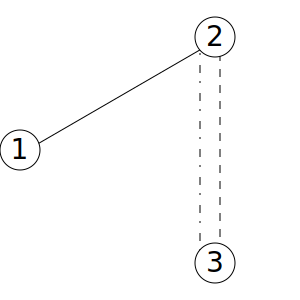
\includegraphics[width=0.3\textwidth]{d3c3_2.pdf}
\end{figure}

A hypothetical fundamental domain is shown on figure \ref{fig:d3c3_2_fundom}.
transparent chamber facets are mirrors, colored facets are glued together. (The
only gluing this fundamental domain has is the $\sigma^1$ adjacency between
$D_2$ and $D_3$.) The wireframe of a parallelepiped is shown to give an idea of
the base of the barycentric subdivision and the vertices of the chambers are
labelled with a number and a set of numbers $i_{\leftsub{c}{\mathcal{D}}^i}$
where $i$ is the label of vertex in the barycentric subdivision and
$\leftsub{c}{\mathcal{D}}^i$ are the chamber-classes having this vertex in
common.

\begin{figure}
  \caption{\label{fig:d3c3_2_fundom} Fundamental domain of d3c3\_2}
  \center
  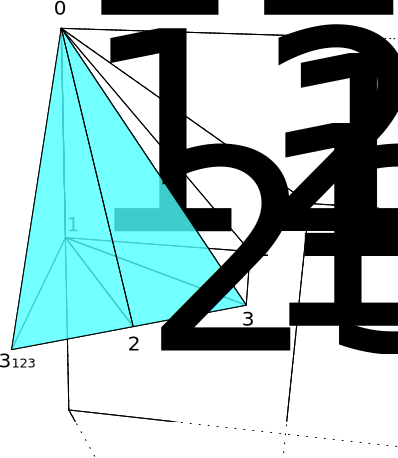
\includegraphics[width=0.6\textwidth]{d3c3_2_fundom.png}
\end{figure}

Figure \ref{fig:d3c3_2_r}. shows the $\mathcal{R}$ matrix function based on the
diagram.\footnote{FIXME olvasora hagyhato, de nagyon hasznos az S3 szignaturak
felirasakor}

\begin{figure}
  \caption{\label{fig:d3c3_2_r} $\mathcal{R}$ matrix function of d3c3\_2}
  \begin{equation*}
    \mathcal{R}(D_1)=
    \left(
    \begin{array}{cccc}
      1 & 1 & 2 & 1\\
      1 & 1 & 3 & 1\\
      2 & 3 & 1 & 3\\
      1 & 1 & 3 & 1
    \end{array}
    \right)
  \end{equation*}
  \begin{equation*}
    \mathcal{R}(D_2)=
    \left(
    \begin{array}{cccc}
      1 & 2 & 2 & 2\\
      2 & 1 & 3 & 1\\
      2 & 3 & 1 & 3\\
      2 & 1 & 3 & 1
    \end{array}
    \right)
  \end{equation*}
  \begin{equation*}
    \mathcal{R}(D_3)=
    \left(
    \begin{array}{cccc}
      1 & 2 & 1 & 2\\
      2 & 1 & 3 & 1\\
      1 & 3 & 1 & 3\\
      2 & 1 & 3 & 1
    \end{array}
    \right)
  \end{equation*}
\end{figure}

Figure \ref{fig:d3c3_2_pm}. shows the parametric $\mathcal{M}$ matrix function
based on the diagram. One can examine that the values are the same around the
edges of the chambers (eg. let $i=0$ and $j=1$, then
$D_1=\sigma^0D_1=\sigma^0\sigma_1D_1$ gets parameter $a$ and $D_2$,
$D_3=\sigma^1D_2$ gets parameter $2b$.) Using the short notation:
$D_1(a,3c,3d)$, $D_2(2b,3c,3d)$, $D_3(2b,3c,3d)$, 

\begin{figure}
  \caption{\label{fig:d3c3_2_pm} Parametric $\mathcal{M}$ matrix function of d3c3\_2}
  \begin{equation*}
    \mathcal{M}(D_1)=
    \left(
    \begin{array}{cccc}
      1 & a & 2 & 2\\
      a & 1 & 3c & 2\\
      2 & 3c & 1 & 3d\\
      2 & 2 & 3d & 1
    \end{array}
    \right)
  \end{equation*}
  \begin{equation*}
    \mathcal{M}(D_2)=
    \left(
    \begin{array}{cccc}
      1 & 2b & 2 & 2\\
      2b & 1 & 3c & 2\\
      2 & 3c & 1 & 3d\\
      2 & 2 & 3d & 1
    \end{array}
    \right)
  \end{equation*}
  \begin{equation*}
    \mathcal{M}(D_3)=
    \left(
    \begin{array}{cccc}
      1 & 2b & 2 & 2\\
      2b & 1 & 3c & 2\\
      2 & 3c & 1 & 3d\\
      2 & 2 & 3d & 1
    \end{array}
    \right)
  \end{equation*}
\end{figure}

Let's consider the case where $b=2$, $c=1$, $d=2$. We'll show that any $a\geq3$ value
gives us a proper D-symbol. Take every D-subsymbol:
\begin{enumerate}
  \setcounter{enumi}{-1}
  \item If we cancel the $0$th adjacency we get a single D-subsymbol, lets
    calculate its combinatorial curvature function:
    \begin{align*}
      K(\leftsub{c}{\mathcal{D}^i})&=\sum_{D\in
      \leftsub{c}{\mathcal{D}^i}}\left(-1+\sum_{\substack{0\le j<k\le d \\ j,k\ne i}}\frac{1}{m^{jk}(D)}\right)= \\
      &
      \sum_{D\in\leftsub{1}{\mathcal{D}^0}}\left(-1+\frac{1}{m^{12}(D)}+\frac{1}{m^{13}(D)}+\frac{1}{m^{23}(D)}\right)= \\
      & -3 + 3\frac{1}{3c} + 3\frac{1}{2} + 3\frac{1}{3d} = -\frac{3}{2}+\frac{1}{c}+\frac{1}{d} = 0
    \end{align*}
    We got a euclidean tiling, which means that the vertex labeled with $0$ must
    be an ideal vertex.
  \item Cancelling the $1$st adjacency results in a single D-subsymbol, which
    shows the edge-transitivity, its curvature function is:
    \begin{align*}
      K(\leftsub{1}{\mathcal{D}^1})&= -3 + 3\frac{1}{2} + 3\frac{1}{2} +
      3\frac{1}{3d} = \frac{1}{d} > 0
    \end{align*}
    Which means we have to check the good orbifold criteria: the signature is
    $*22d$ which is a good orbifold (even for $d=1$), so this must be a proper vertex.
  \item Cancelling the $2$nd adjacency the curvature functions are:
    \begin{align*}
      K(\leftsub{1}{\mathcal{D}^2})&= -1 + \frac{1}{2} + \frac{1}{2} +
      \frac{1}{a} = \frac{1}{a} > 0
    \end{align*}
    Which means we have to check the good orbifold criteria: the signature is
    $*22a$, good orbifold, proper vertex.
    \begin{align*}
      K(\leftsub{2}{\mathcal{D}^2})&= -2 + 2\frac{1}{2} + 2\frac{1}{2} +
      2\frac{1}{2b} = \frac{1}{b} > 0
    \end{align*}
    The signature is $2*b$, good orbifold, proper vertex if $b\geq2$, which is
    the case.
  \item Cancelling the $3$rd adjacency the curvature function is:
    \begin{align*}
      K(\leftsub{1}{\mathcal{D}^3})&= -3 + 3\frac{1}{2} + \frac{1}{a} +
      2\frac{1}{2b} + 3\frac{1}{3c} =
       -\frac{3}{2} + \frac{1}{b} + \frac{1}{c} + \frac{1}{a} > 0
    \end{align*}
    If $b=2$ and $c=1$, then for any value of $a$ the above formula is positive.
    The signature is $*22ac$, good orbifold proper vertex.
\end{enumerate}

%FIXME Splitting?

%\begin{figure}
%  \caption{}
%\end{figure}


%Start with cardinality 24 as there are maximal examples, but go down to
%cardinality 6 or 3 so it's easier to see... Graphics

%R matrix functions. Some possible M matrix functions (maximal, non max): Let's
%see a sphere's curvature function around a vertex (smaller cardinality?).

%(Non-)maximality example. d3c6\_13

Let's see another $3$-dimensional example but with cardinality $6$. The
D-diagram with the possible homomorphisms is shown in Fig.
\ref{fig:d3c6_13}.

\begin{figure}
  \caption{\label{fig:d3c6_13} D-diagram of d3c6\_13, loops are not indicated}
  \center
  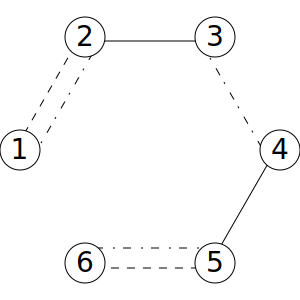
\includegraphics[width=0.3\textwidth]{d3c6_13.pdf}
\end{figure}

A hypothetical fundamental domain is shown on figure \ref{fig:d3c6_13_fundom}.
transparent chamber facets are mirrors, colored facets are glued together.
(There are $2$ gluing operations in this fundamental domain: the $\sigma^1$ adjacency between
$D_1$ and $D_2$, and between $D_5$ and $D_6$.)

\begin{figure}
  \caption{\label{fig:d3c6_13_fundom} Fundamental domain of d3c6\_13}
  \center
  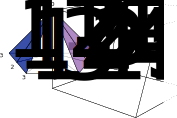
\includegraphics[width=0.6\textwidth]{d3c6_13_fundom.png}
\end{figure}

Calculating the $\mathcal{R}$ matrix function is left to the reader as an
exercise.

The short version of the parametric $\mathcal{M}$ matrix function based on the
diagram: $D_1(2a, 3e, 6g)$, $D_2(2a, 3e, 6g)$, $D_3(b, 3e, 6g)$, $D_4(c, 3f,
6g)$, $D_5(2d, 3f, 6g)$, $D_6(2d, 3f, 6g)$.

The combinatorial curvature function can be calculated for every D-subsymbol,
let's consider the case where
$D_3,D_4\in\leftsub{c}{(\Sigma^I,\mathcal{D}_2,\mathcal{M}_2)}$. The combinatorial
curvature function leads to a positive value, but if we take the signature of
the D-subsymbol we get $*bc$ ($b,c>1$), which means that $b=c$ must hold or else
we get a bad orbifold.

Let's take the following valid parameter values: $a=2$, $d=2$, $e=1$, $f=1$, $g=1$ and
an arbitrary value for $b=c\geq3$. Let's take a homomorphism $\phi$ with
$Ker(\phi)={D_1,D_6}$. It's easy to see, that this homomorphism unites $D_1$
with $D_6$, $D_2$ with $D_5$ and $D_3$ with $D_4$. The adjacency operations and
the $\mathcal{M}$ matrix function act nicely on the resulting D-symbol
with cardinality $3$ which is isomorphic to our previous example (up to a
permutation). This means that this D-symbol is non-maximal, but a symmetry
breaking of the previous one. 

If we take another set of valid parameter values: $a=2$, $b=c=3$, $d=3$, $e=1$,
$f=1$, $g=1$ the resulting D-symbol is maximal, because the homomorphisms of the
D-diagram cannot be extended to the $\mathcal{M}$ matrix functions.

As was mentioned in section \ref{sec:edge_transitive} the biggest edge
transitive D-symbols have a cardinality of $24$, let's see an example:
The D-diagram with the possible homomorphisms is shown in Fig.
\ref{fig:d3c24_2}.

\begin{figure}
  \caption{\label{fig:d3c24_2} D-diagram of d3c24\_2}
  \center
  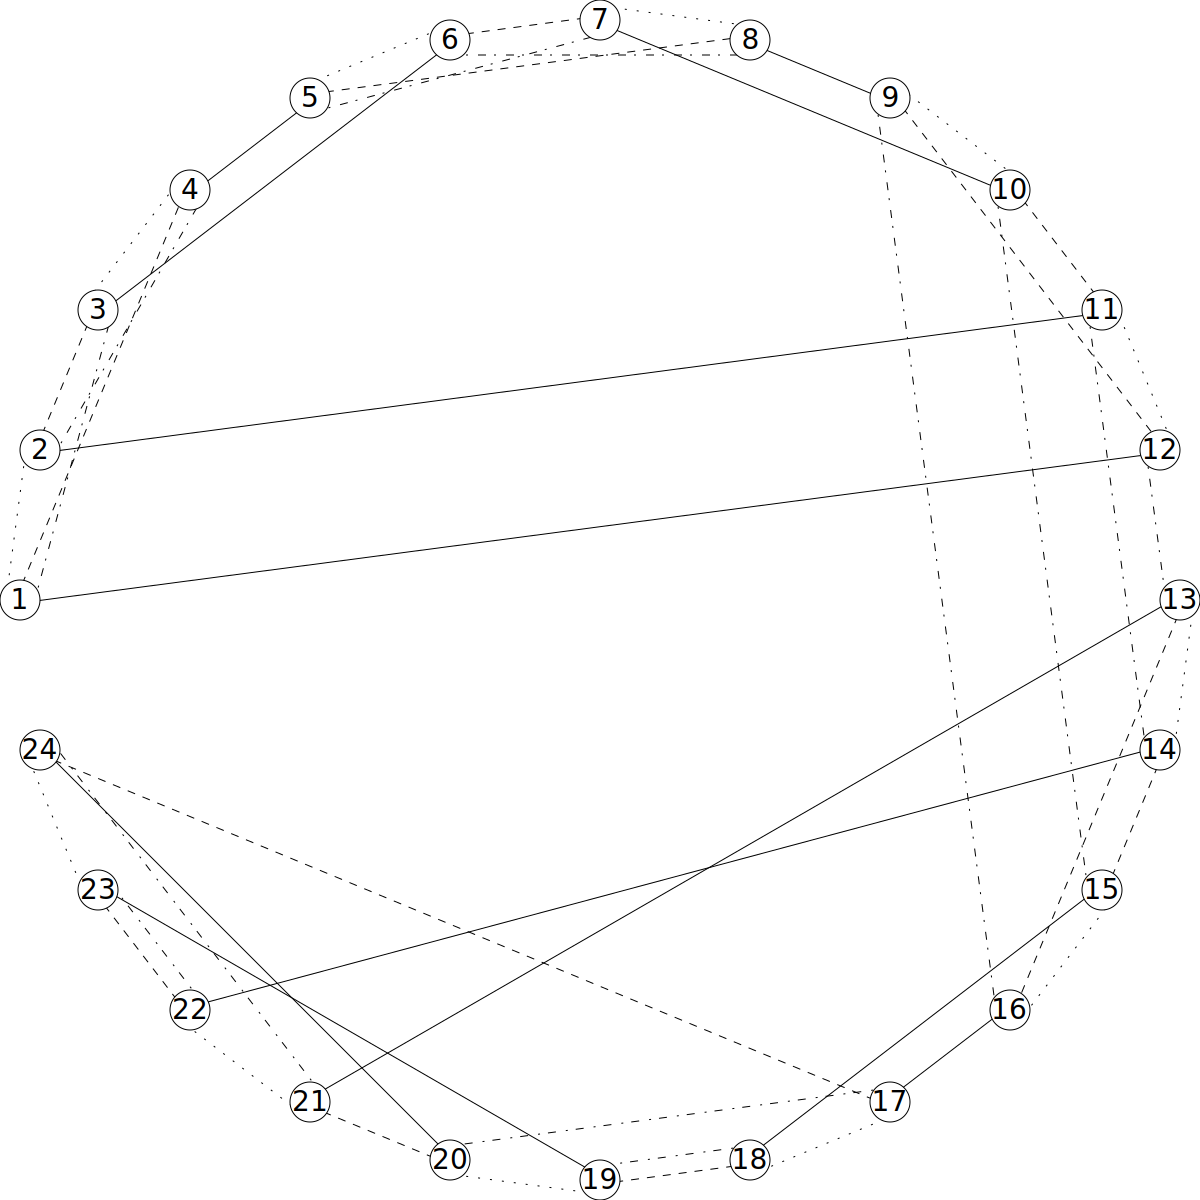
\includegraphics[width=0.8\textwidth]{d3c24_2.pdf}
\end{figure}

A hypothetical fundamental domain is shown on figure \ref{fig:d3c24_2_fundom}.

\begin{figure}
  \caption{\label{fig:d3c24_2_fundom} Fundamental domain of d3c24\_2}
  \center
  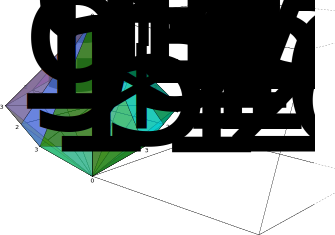
\includegraphics[width=1\textwidth]{d3c24_2_fundom.png}
\end{figure}

The short version of the parametric $\mathcal{M}$ matrix function based on the
diagram (after good orbifold checks): $D_1(2a, 3f, 6k)$, $D_2(2a, 3g, 6k)$,
$D_3(2a, 3g, 6k)$, $D_4(2a, 3f, 6k)$, $D_5(2b, 3f, 6k)$, $D_6(2b, 3g, 6k)$,
$D_7(2b, 3g, 6k)$, $D_8(2b, 3f, 6k)$, $D_9(2c, 3f, 6k)$, $D_{10}(2c, 3g, 6k)$,
$D_{11}(2c, 3g, 6k)$, $D_{12}(2c, 3f, 6k)$, $D_{13}(2c, 3h, 6k)$, $D_{14}(2c,
3i, 6k)$, $D_{15}(2c, 3i, 6k)$, $D_{16}(2c, 3h, 6k)$, $D_{17}(4e, 3h, 6k)$,
$D_{18}(4e, 3i, 6k)$, $D_{19}(4e, 3i, 6k)$, $D_{20}(4e, 3h, 6k)$, $D_{21}(4e,
3h, 6k)$, $D_{22}(4e, 3i, 6k)$, $D_{23}(4e, 3i, 6k)$, $D_{24}(4e, 3h, 6k)$.

If we take the valid parameter values: $a=b=2$, $e=f=g=h=i=k=1$ and any value
for $c\geq2$, then the D-symbol is non-maximal, every homomorphism of the
D-diagram shown in Fig. \ref{fig:d3c24_2} is also a homomorphism of the D-symbol
(including the $\mathcal{M}$ matrix function) and we got a symmetry breaking of
our first example (Fig. \ref{fig:d3c3_2}).

If we take another valid parameter set: $a=c=2$, $e=f=g=h=i=k=1$ and any value
for $b\geq3$\footnote{the case where $b=2$ is contained in the previous set},
then the D-symbol is maximal.

\section{Future work}
Analyse every edge-transitive symbol

Check 2 dimensional tilings on the border of partitions (splitting/fiber)

Difficult part: find out the signature and type of underlying geometries

\section{Acknowledgement}


%Bibiliography
\nocite{DHM93,D87,Du88,H93,LM90,Ma67,M94,T82,VS93,F94,M11,DDH98,K11}
\bibliographystyle{plain}
\bibliography{dsym}

\end{document}
